\documentclass[11pt, a4paper]{article}\usepackage[]{graphicx}\usepackage[]{xcolor}
% maxwidth is the original width if it is less than linewidth
% otherwise use linewidth (to make sure the graphics do not exceed the margin)
\makeatletter
\def\maxwidth{ %
  \ifdim\Gin@nat@width>\linewidth
    \linewidth
  \else
    \Gin@nat@width
  \fi
}
\makeatother

\definecolor{fgcolor}{rgb}{0.345, 0.345, 0.345}
\newcommand{\hlnum}[1]{\textcolor[rgb]{0.686,0.059,0.569}{#1}}%
\newcommand{\hlsng}[1]{\textcolor[rgb]{0.192,0.494,0.8}{#1}}%
\newcommand{\hlcom}[1]{\textcolor[rgb]{0.678,0.584,0.686}{\textit{#1}}}%
\newcommand{\hlopt}[1]{\textcolor[rgb]{0,0,0}{#1}}%
\newcommand{\hldef}[1]{\textcolor[rgb]{0.345,0.345,0.345}{#1}}%
\newcommand{\hlkwa}[1]{\textcolor[rgb]{0.161,0.373,0.58}{\textbf{#1}}}%
\newcommand{\hlkwb}[1]{\textcolor[rgb]{0.69,0.353,0.396}{#1}}%
\newcommand{\hlkwc}[1]{\textcolor[rgb]{0.333,0.667,0.333}{#1}}%
\newcommand{\hlkwd}[1]{\textcolor[rgb]{0.737,0.353,0.396}{\textbf{#1}}}%
\let\hlipl\hlkwb

\usepackage{framed}
\makeatletter
\newenvironment{kframe}{%
 \def\at@end@of@kframe{}%
 \ifinner\ifhmode%
  \def\at@end@of@kframe{\end{minipage}}%
  \begin{minipage}{\columnwidth}%
 \fi\fi%
 \def\FrameCommand##1{\hskip\@totalleftmargin \hskip-\fboxsep
 \colorbox{shadecolor}{##1}\hskip-\fboxsep
     % There is no \\@totalrightmargin, so:
     \hskip-\linewidth \hskip-\@totalleftmargin \hskip\columnwidth}%
 \MakeFramed {\advance\hsize-\width
   \@totalleftmargin\z@ \linewidth\hsize
   \@setminipage}}%
 {\par\unskip\endMakeFramed%
 \at@end@of@kframe}
\makeatother

\definecolor{shadecolor}{rgb}{.97, .97, .97}
\definecolor{messagecolor}{rgb}{0, 0, 0}
\definecolor{warningcolor}{rgb}{1, 0, 1}
\definecolor{errorcolor}{rgb}{1, 0, 0}
\newenvironment{knitrout}{}{} % an empty environment to be redefined in TeX

\usepackage{alltt}

\usepackage[top = 0.6 in, bottom = 0.7 in, left = 1 in, right = 1 in]{geometry}

\usepackage{amsmath, amssymb, amsfonts}
\usepackage{enumerate}
\usepackage{array}
\usepackage{multirow}
\usepackage{dingbat}
\usepackage{fontawesome5}
\usepackage{tasks}
\usepackage{bbding}
\usepackage{twemojis}
% how to use bull's eye ----- \scalebox{2.0}{\twemoji{bullseye}}
\usepackage{fontspec}
\usepackage{customdice}
% how to put dice face ------ \dice{2}

\title{MSMS 308 : Practical 02}
\author{Ananda Biswas}
\date{\today}

\newfontface\myfont{Myfont1-Regular.ttf}[LetterSpace=0.05em]
% how to use ---- {\setlength{\spaceskip}{1em plus 0.5em minus 0.5em} \fontsize{17}{20}\myfont --write text here-- \par}

\newfontface\cbfont{CaveatBrush-Regular.ttf}
% how to use --- \myfont --write text here--
\IfFileExists{upquote.sty}{\usepackage{upquote}}{}
\begin{document}

\maketitle


\section*{\faArrowAltCircleRight[regular] \textcolor{blue}{Question}}

\hspace{1cm} Generate random numbers using the Exponential distribution with rate parameter $\lambda$. Perform the following tasks:
\begin{enumerate}
\item Generate data-sets of sizes 30, 50, and 100 using function in R.
\item For each sample, estimate the rate parameter $\lambda$ using Maximum Likelihood Estimation.
\item Using the estimated parameter, compute and plot the following functions:
  \begin{enumerate}[(a)]
  \item Probability Density Function $f(t)$
  \item Survival Function $S(t)$
  \item Hazard Function $h(t)$
  \item Cumulative Hazard Function $H(t)$.
  \end{enumerate}
\item Compare how the shape and values of these functions change with different sample sizes.
\end{enumerate}


\section*{\faArrowAltCircleRight[regular] \textcolor{blue}{Theory}}

The probability distribution function of a lifetime $T$ having Exponential Distribution with rate $\lambda > 0$ is 
$$f(t) = \lambda e^{-\lambda t} \cdot I_{(0, \infty)}(t).$$\\

The Survival Function is $S(t) = e^{-\lambda t} \,\, \forall t > 0$.\\[0.5em]

The Hazard Function is $h(t) = \lambda \,\, \forall t > 0$.\\[0.5em]

The Cumulative Hazard Function is $H(t) = \lambda t \,\, \forall t > 0$.\\[0.5em]

By the method of Maximum Likelihood Estimation, $\hat{\lambda} = \dfrac{1}{\overline{T}}$.

\section*{\faArrowAltCircleRight[regular] \textcolor{blue}{R Program}}

\begin{knitrout}
\definecolor{shadecolor}{rgb}{0.969, 0.969, 0.969}\color{fgcolor}\begin{kframe}
\begin{alltt}
\hldef{f_t} \hlkwb{<-} \hlkwa{function}\hldef{(}\hlkwc{t}\hldef{,} \hlkwc{lambda}\hldef{) lambda} \hlopt{*} \hlkwd{exp}\hldef{(}\hlopt{-}\hldef{lambda} \hlopt{*} \hldef{t)}
\hldef{S_t} \hlkwb{<-} \hlkwa{function}\hldef{(}\hlkwc{t}\hldef{,} \hlkwc{lambda}\hldef{)} \hlkwd{exp}\hldef{(}\hlopt{-}\hldef{lambda} \hlopt{*} \hldef{t)}
\hldef{h_t} \hlkwb{<-} \hlkwa{function}\hldef{(}\hlkwc{t}\hldef{,} \hlkwc{lambda}\hldef{) lambda}
\hldef{H_t} \hlkwb{<-} \hlkwa{function}\hldef{(}\hlkwc{t}\hldef{,} \hlkwc{lambda}\hldef{) lambda} \hlopt{*} \hldef{t}
\end{alltt}
\end{kframe}
\end{knitrout}

\newpage




\dice{1} $n = 30$.

\begin{knitrout}
\definecolor{shadecolor}{rgb}{0.969, 0.969, 0.969}\color{fgcolor}\begin{kframe}
\begin{alltt}
\hldef{n} \hlkwb{<-} \hlnum{30}
\end{alltt}
\end{kframe}
\end{knitrout}

\begin{knitrout}
\definecolor{shadecolor}{rgb}{0.969, 0.969, 0.969}\color{fgcolor}\begin{kframe}
\begin{alltt}
\hldef{s} \hlkwb{<-} \hlkwd{rexp}\hldef{(n,} \hlkwc{rate} \hldef{=} \hlnum{0.5}\hldef{)}
\end{alltt}
\end{kframe}
\end{knitrout}

\begin{knitrout}
\definecolor{shadecolor}{rgb}{0.969, 0.969, 0.969}\color{fgcolor}\begin{kframe}
\begin{alltt}
\hldef{lambda_hat} \hlkwb{<-} \hlnum{1} \hlopt{/} \hlkwd{mean}\hldef{(s); lambda_hat}
\end{alltt}
\begin{verbatim}
## [1] 0.4611669
\end{verbatim}
\end{kframe}
\end{knitrout}

\begin{knitrout}
\definecolor{shadecolor}{rgb}{0.969, 0.969, 0.969}\color{fgcolor}\begin{kframe}
\begin{alltt}
\hldef{df1} \hlkwb{<-} \hlkwd{data.frame}\hldef{(}\hlkwc{t} \hldef{= s,}
                  \hlkwc{f_t_hat} \hldef{=} \hlkwd{f_t}\hldef{(s, lambda_hat),}
                  \hlkwc{S_t_hat} \hldef{=} \hlkwd{S_t}\hldef{(s, lambda_hat),}
                  \hlkwc{h_t_hat} \hldef{=} \hlkwd{h_t}\hldef{(s, lambda_hat),}
                  \hlkwc{H_t_hat} \hldef{=} \hlkwd{H_t}\hldef{(s, lambda_hat))}
\end{alltt}
\end{kframe}
\end{knitrout}


\dice{2} $n = 50$.

\begin{knitrout}
\definecolor{shadecolor}{rgb}{0.969, 0.969, 0.969}\color{fgcolor}\begin{kframe}
\begin{alltt}
\hldef{n} \hlkwb{<-} \hlnum{50}
\end{alltt}
\end{kframe}
\end{knitrout}

\begin{knitrout}
\definecolor{shadecolor}{rgb}{0.969, 0.969, 0.969}\color{fgcolor}\begin{kframe}
\begin{alltt}
\hldef{s} \hlkwb{<-} \hlkwd{rexp}\hldef{(n,} \hlkwc{rate} \hldef{=} \hlnum{0.5}\hldef{)}
\end{alltt}
\end{kframe}
\end{knitrout}

\begin{knitrout}
\definecolor{shadecolor}{rgb}{0.969, 0.969, 0.969}\color{fgcolor}\begin{kframe}
\begin{alltt}
\hldef{lambda_hat} \hlkwb{<-} \hlnum{1} \hlopt{/} \hlkwd{mean}\hldef{(s); lambda_hat}
\end{alltt}
\begin{verbatim}
## [1] 0.4625597
\end{verbatim}
\end{kframe}
\end{knitrout}

\begin{knitrout}
\definecolor{shadecolor}{rgb}{0.969, 0.969, 0.969}\color{fgcolor}\begin{kframe}
\begin{alltt}
\hldef{df2} \hlkwb{<-} \hlkwd{data.frame}\hldef{(}\hlkwc{t} \hldef{= s,}
                  \hlkwc{f_t_hat} \hldef{=} \hlkwd{f_t}\hldef{(s, lambda_hat),}
                  \hlkwc{S_t_hat} \hldef{=} \hlkwd{S_t}\hldef{(s, lambda_hat),}
                  \hlkwc{h_t_hat} \hldef{=} \hlkwd{h_t}\hldef{(s, lambda_hat),}
                  \hlkwc{H_t_hat} \hldef{=} \hlkwd{H_t}\hldef{(s, lambda_hat))}
\end{alltt}
\end{kframe}
\end{knitrout}

\dice{3} $n = 100$.

\begin{knitrout}
\definecolor{shadecolor}{rgb}{0.969, 0.969, 0.969}\color{fgcolor}\begin{kframe}
\begin{alltt}
\hldef{n} \hlkwb{<-} \hlnum{100}
\end{alltt}
\end{kframe}
\end{knitrout}

\begin{knitrout}
\definecolor{shadecolor}{rgb}{0.969, 0.969, 0.969}\color{fgcolor}\begin{kframe}
\begin{alltt}
\hldef{s} \hlkwb{<-} \hlkwd{rexp}\hldef{(n,} \hlkwc{rate} \hldef{=} \hlnum{0.5}\hldef{)}
\end{alltt}
\end{kframe}
\end{knitrout}

\begin{knitrout}
\definecolor{shadecolor}{rgb}{0.969, 0.969, 0.969}\color{fgcolor}\begin{kframe}
\begin{alltt}
\hldef{lambda_hat} \hlkwb{<-} \hlnum{1} \hlopt{/} \hlkwd{mean}\hldef{(s); lambda_hat}
\end{alltt}
\begin{verbatim}
## [1] 0.5050291
\end{verbatim}
\end{kframe}
\end{knitrout}

\begin{knitrout}
\definecolor{shadecolor}{rgb}{0.969, 0.969, 0.969}\color{fgcolor}\begin{kframe}
\begin{alltt}
\hldef{df3} \hlkwb{<-} \hlkwd{data.frame}\hldef{(}\hlkwc{t} \hldef{= s,}
                  \hlkwc{f_t_hat} \hldef{=} \hlkwd{f_t}\hldef{(s, lambda_hat),}
                  \hlkwc{S_t_hat} \hldef{=} \hlkwd{S_t}\hldef{(s, lambda_hat),}
                  \hlkwc{h_t_hat} \hldef{=} \hlkwd{h_t}\hldef{(s, lambda_hat),}
                  \hlkwc{H_t_hat} \hldef{=} \hlkwd{H_t}\hldef{(s, lambda_hat))}
\end{alltt}
\end{kframe}
\end{knitrout}

\newpage

\section*{\faArrowAltCircleRight[regular] \textcolor{blue}{Plots}}



\dice{1} $n = 30$.

\begin{knitrout}
\definecolor{shadecolor}{rgb}{0.969, 0.969, 0.969}\color{fgcolor}\begin{kframe}
\begin{alltt}
\hldef{p1} \hlkwb{<-} \hldef{df1} \hlopt
        \hlkwd{ggplot}\hldef{(}\hlkwd{aes}\hldef{(}\hlkwc{x} \hldef{= t,} \hlkwc{y} \hldef{= f_t_hat))} \hlopt{+} \hlkwd{geom_point}\hldef{(}\hlkwc{col} \hldef{=} \hlsng{"blue"}\hldef{)} \hlopt{+}
        \hlkwd{labs}\hldef{(}\hlkwc{x} \hldef{=} \hlsng{"t"}\hldef{,} \hlkwc{y} \hldef{=} \hlsng{"f(t)"}\hldef{,} \hlkwc{title} \hldef{=} \hlsng{"Estimated PDF"}\hldef{)}

\hldef{p2} \hlkwb{<-} \hldef{df1} \hlopt
        \hlkwd{ggplot}\hldef{(}\hlkwd{aes}\hldef{(}\hlkwc{x} \hldef{= t,} \hlkwc{y} \hldef{= S_t_hat))} \hlopt{+} \hlkwd{geom_point}\hldef{(}\hlkwc{col} \hldef{=} \hlsng{"blue"}\hldef{)} \hlopt{+}
        \hlkwd{labs}\hldef{(}\hlkwc{x} \hldef{=} \hlsng{"t"}\hldef{,} \hlkwc{y} \hldef{=} \hlsng{"S(t)"}\hldef{,} \hlkwc{title} \hldef{=} \hlsng{"Estimated Survival Function"}\hldef{)}

\hldef{p3} \hlkwb{<-} \hldef{df1} \hlopt
        \hlkwd{ggplot}\hldef{(}\hlkwd{aes}\hldef{(}\hlkwc{x} \hldef{= t,} \hlkwc{y} \hldef{= h_t_hat))} \hlopt{+} \hlkwd{geom_point}\hldef{(}\hlkwc{col} \hldef{=} \hlsng{"blue"}\hldef{)} \hlopt{+}
        \hlkwd{labs}\hldef{(}\hlkwc{x} \hldef{=} \hlsng{"t"}\hldef{,} \hlkwc{y} \hldef{=} \hlsng{"h(t)"}\hldef{,} \hlkwc{title} \hldef{=} \hlsng{"Estimated Hazard Function"}\hldef{)}

\hldef{p4} \hlkwb{<-} \hldef{df1} \hlopt
        \hlkwd{ggplot}\hldef{(}\hlkwd{aes}\hldef{(}\hlkwc{x} \hldef{= t,} \hlkwc{y} \hldef{= H_t_hat))} \hlopt{+} \hlkwd{geom_point}\hldef{(}\hlkwc{col} \hldef{=} \hlsng{"blue"}\hldef{)} \hlopt{+}
        \hlkwd{labs}\hldef{(}\hlkwc{x} \hldef{=} \hlsng{"t"}\hldef{,} \hlkwc{y} \hldef{=} \hlsng{"H(t)"}\hldef{,} \hlkwc{title} \hldef{=} \hlsng{"Estimated Cumulative Hazard Function"}\hldef{)}
\end{alltt}
\end{kframe}
\end{knitrout}

\begin{knitrout}
\definecolor{shadecolor}{rgb}{0.969, 0.969, 0.969}\color{fgcolor}\begin{kframe}
\begin{alltt}
\hlkwd{grid.arrange}\hldef{(p1, p2, p3, p4,} \hlkwc{ncol} \hldef{=} \hlnum{2}\hldef{)}
\end{alltt}
\end{kframe}
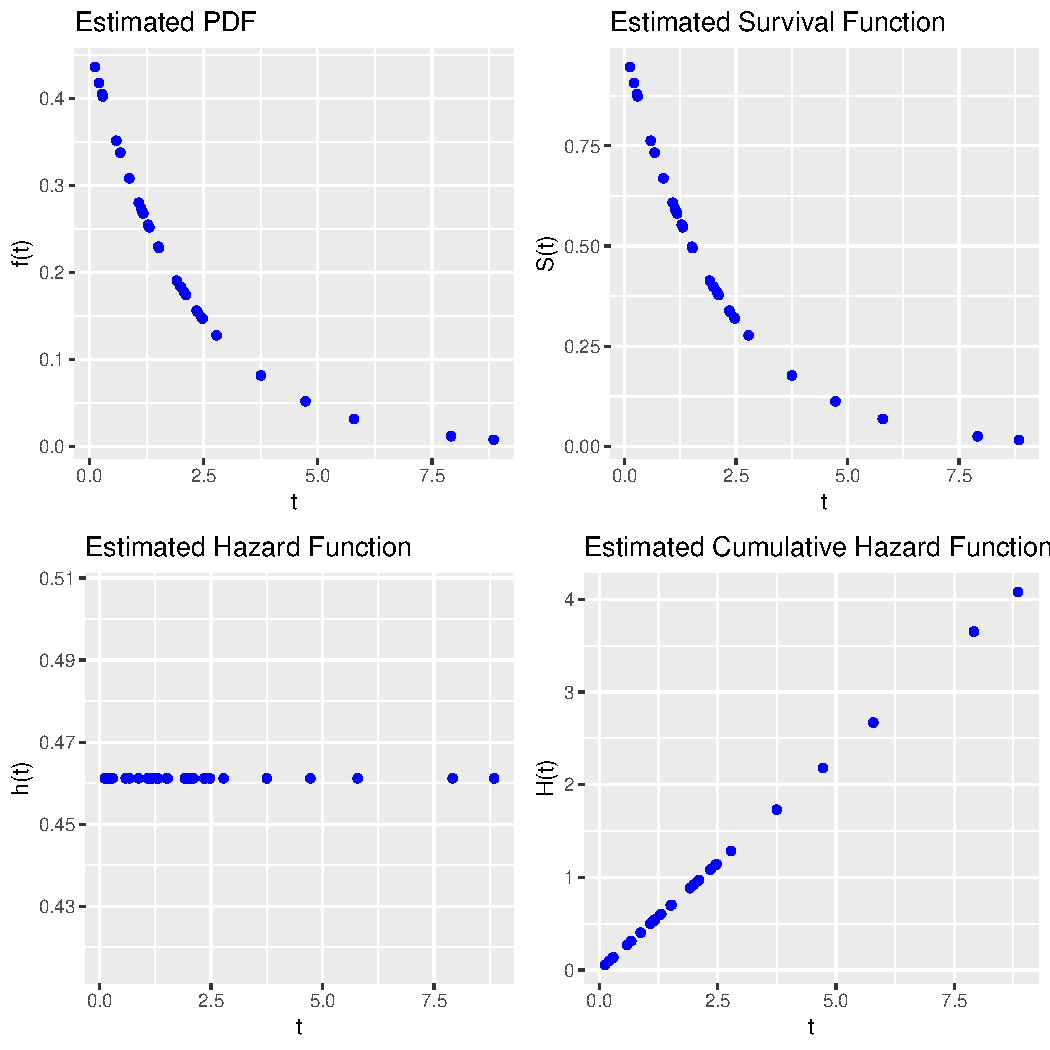
\includegraphics[width=\maxwidth]{figure/unnamed-chunk-17-1} 
\end{knitrout}

\dice{2} $n = 50$.

\begin{knitrout}
\definecolor{shadecolor}{rgb}{0.969, 0.969, 0.969}\color{fgcolor}\begin{kframe}
\begin{alltt}
\hldef{p1} \hlkwb{<-} \hldef{df2} \hlopt
        \hlkwd{ggplot}\hldef{(}\hlkwd{aes}\hldef{(}\hlkwc{x} \hldef{= t,} \hlkwc{y} \hldef{= f_t_hat))} \hlopt{+} \hlkwd{geom_point}\hldef{(}\hlkwc{col} \hldef{=} \hlsng{"blue"}\hldef{)} \hlopt{+}
        \hlkwd{labs}\hldef{(}\hlkwc{x} \hldef{=} \hlsng{"t"}\hldef{,} \hlkwc{y} \hldef{=} \hlsng{"f(t)"}\hldef{,} \hlkwc{title} \hldef{=} \hlsng{"Estimated PDF"}\hldef{)}

\hldef{p2} \hlkwb{<-} \hldef{df2} \hlopt
        \hlkwd{ggplot}\hldef{(}\hlkwd{aes}\hldef{(}\hlkwc{x} \hldef{= t,} \hlkwc{y} \hldef{= S_t_hat))} \hlopt{+} \hlkwd{geom_point}\hldef{(}\hlkwc{col} \hldef{=} \hlsng{"blue"}\hldef{)} \hlopt{+}
        \hlkwd{labs}\hldef{(}\hlkwc{x} \hldef{=} \hlsng{"t"}\hldef{,} \hlkwc{y} \hldef{=} \hlsng{"S(t)"}\hldef{,} \hlkwc{title} \hldef{=} \hlsng{"Estimated Survival Function"}\hldef{)}

\hldef{p3} \hlkwb{<-} \hldef{df2} \hlopt
        \hlkwd{ggplot}\hldef{(}\hlkwd{aes}\hldef{(}\hlkwc{x} \hldef{= t,} \hlkwc{y} \hldef{= h_t_hat))} \hlopt{+} \hlkwd{geom_point}\hldef{(}\hlkwc{col} \hldef{=} \hlsng{"blue"}\hldef{)} \hlopt{+}
        \hlkwd{labs}\hldef{(}\hlkwc{x} \hldef{=} \hlsng{"t"}\hldef{,} \hlkwc{y} \hldef{=} \hlsng{"h(t)"}\hldef{,} \hlkwc{title} \hldef{=} \hlsng{"Estimated Hazard Function"}\hldef{)}

\hldef{p4} \hlkwb{<-} \hldef{df2} \hlopt
        \hlkwd{ggplot}\hldef{(}\hlkwd{aes}\hldef{(}\hlkwc{x} \hldef{= t,} \hlkwc{y} \hldef{= H_t_hat))} \hlopt{+} \hlkwd{geom_point}\hldef{(}\hlkwc{col} \hldef{=} \hlsng{"blue"}\hldef{)} \hlopt{+}
        \hlkwd{labs}\hldef{(}\hlkwc{x} \hldef{=} \hlsng{"t"}\hldef{,} \hlkwc{y} \hldef{=} \hlsng{"H(t)"}\hldef{,} \hlkwc{title} \hldef{=} \hlsng{"Estimated Cumulative Hazard Function"}\hldef{)}
\end{alltt}
\end{kframe}
\end{knitrout}

\begin{knitrout}
\definecolor{shadecolor}{rgb}{0.969, 0.969, 0.969}\color{fgcolor}\begin{kframe}
\begin{alltt}
\hlkwd{grid.arrange}\hldef{(p1, p2, p3, p4,} \hlkwc{ncol} \hldef{=} \hlnum{2}\hldef{)}
\end{alltt}
\end{kframe}
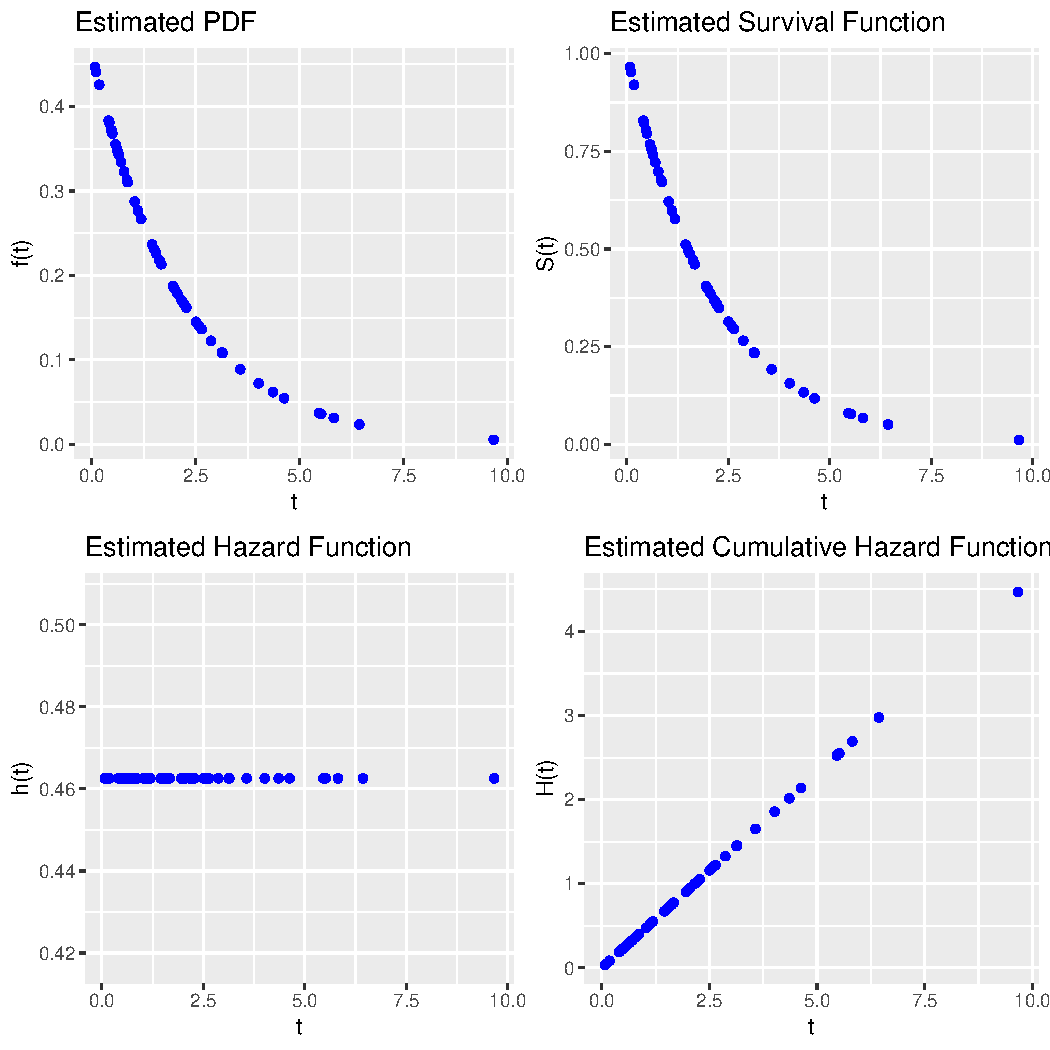
\includegraphics[width=\maxwidth]{figure/unnamed-chunk-19-1} 
\end{knitrout}


\newpage

\dice{3} $n = 100$.

\begin{knitrout}
\definecolor{shadecolor}{rgb}{0.969, 0.969, 0.969}\color{fgcolor}\begin{kframe}
\begin{alltt}
\hldef{p1} \hlkwb{<-} \hldef{df3} \hlopt
        \hlkwd{ggplot}\hldef{(}\hlkwd{aes}\hldef{(}\hlkwc{x} \hldef{= t,} \hlkwc{y} \hldef{= f_t_hat))} \hlopt{+} \hlkwd{geom_point}\hldef{(}\hlkwc{col} \hldef{=} \hlsng{"blue"}\hldef{)} \hlopt{+}
        \hlkwd{labs}\hldef{(}\hlkwc{x} \hldef{=} \hlsng{"t"}\hldef{,} \hlkwc{y} \hldef{=} \hlsng{"f(t)"}\hldef{,} \hlkwc{title} \hldef{=} \hlsng{"Estimated PDF"}\hldef{)}

\hldef{p2} \hlkwb{<-} \hldef{df3} \hlopt
        \hlkwd{ggplot}\hldef{(}\hlkwd{aes}\hldef{(}\hlkwc{x} \hldef{= t,} \hlkwc{y} \hldef{= S_t_hat))} \hlopt{+} \hlkwd{geom_point}\hldef{(}\hlkwc{col} \hldef{=} \hlsng{"blue"}\hldef{)} \hlopt{+}
        \hlkwd{labs}\hldef{(}\hlkwc{x} \hldef{=} \hlsng{"t"}\hldef{,} \hlkwc{y} \hldef{=} \hlsng{"S(t)"}\hldef{,} \hlkwc{title} \hldef{=} \hlsng{"Estimated Survival Function"}\hldef{)}

\hldef{p3} \hlkwb{<-} \hldef{df3} \hlopt
        \hlkwd{ggplot}\hldef{(}\hlkwd{aes}\hldef{(}\hlkwc{x} \hldef{= t,} \hlkwc{y} \hldef{= h_t_hat))} \hlopt{+} \hlkwd{geom_point}\hldef{(}\hlkwc{col} \hldef{=} \hlsng{"blue"}\hldef{)} \hlopt{+}
        \hlkwd{labs}\hldef{(}\hlkwc{x} \hldef{=} \hlsng{"t"}\hldef{,} \hlkwc{y} \hldef{=} \hlsng{"h(t)"}\hldef{,} \hlkwc{title} \hldef{=} \hlsng{"Estimated Hazard Function"}\hldef{)}

\hldef{p4} \hlkwb{<-} \hldef{df3} \hlopt
        \hlkwd{ggplot}\hldef{(}\hlkwd{aes}\hldef{(}\hlkwc{x} \hldef{= t,} \hlkwc{y} \hldef{= H_t_hat))} \hlopt{+} \hlkwd{geom_point}\hldef{(}\hlkwc{col} \hldef{=} \hlsng{"blue"}\hldef{)} \hlopt{+}
        \hlkwd{labs}\hldef{(}\hlkwc{x} \hldef{=} \hlsng{"t"}\hldef{,} \hlkwc{y} \hldef{=} \hlsng{"H(t)"}\hldef{,} \hlkwc{title} \hldef{=} \hlsng{"Estimated Cumulative Hazard Function"}\hldef{)}
\end{alltt}
\end{kframe}
\end{knitrout}

\begin{knitrout}
\definecolor{shadecolor}{rgb}{0.969, 0.969, 0.969}\color{fgcolor}\begin{kframe}
\begin{alltt}
\hlkwd{grid.arrange}\hldef{(p1, p2, p3, p4,} \hlkwc{ncol} \hldef{=} \hlnum{2}\hldef{)}
\end{alltt}
\end{kframe}
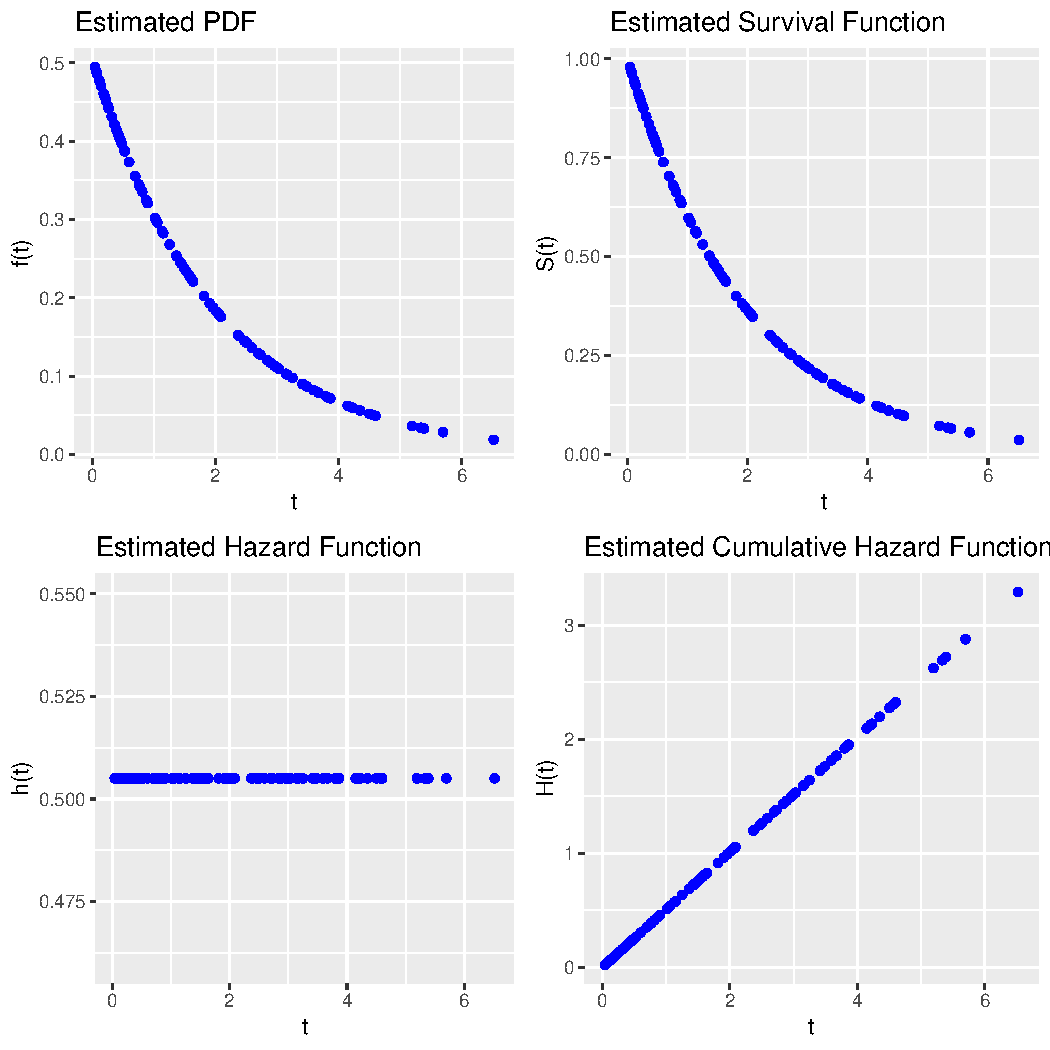
\includegraphics[width=\maxwidth]{figure/unnamed-chunk-21-1} 
\end{knitrout}

\section*{\faArrowAltCircleRight[regular] \textcolor{blue}{Conclusion}}

As the sample size increases, the ML estimate of $\lambda$ becomes less noisy. Consequently the estimated PDF, Survival Function, Hazard Function and Cumulative Hazard match with true shapes of these functions more closely.

\end{document}
